\section{Application au jeu de Pong}

Pour appliquer l'algorithme Acteur-Critique au jeu de Pong nous avons pris pour référence le code source
de \emph{Learning to Play with Pong}\cite{PongGithub}. Ce repository propose une implémentation de la version Advantage Actor-Critic (A2C)
que nous avons adapté à la nouvelle api de gymnasium.

Nous avons par la suite tenté plusieurs modifications dans le but d'améliorer les performances de l'algorithme.
Pour les évaluer, nous avons analysé l'évolution de la moyenne mobile des gains par épisode.
Chaque entrainement a été effectué sur 300 épisodes et a duré en moyenne 3 heures. Bien que le nombre d'épisode nécessaire
pour vaincre l'IA soit plus élevé, nous avons choisit un nombre d'épisode nous permettant d'entrainer plusieurs modèles pour pouvoir ainsi les comparer.
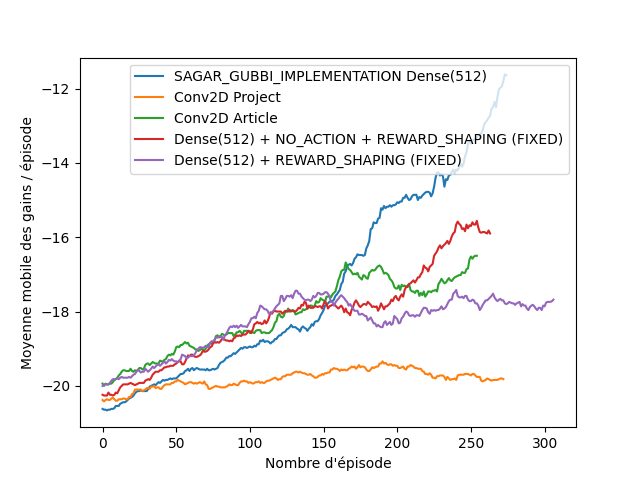
\includegraphics[width=\linewidth]{rolling_average_graph.png}
% 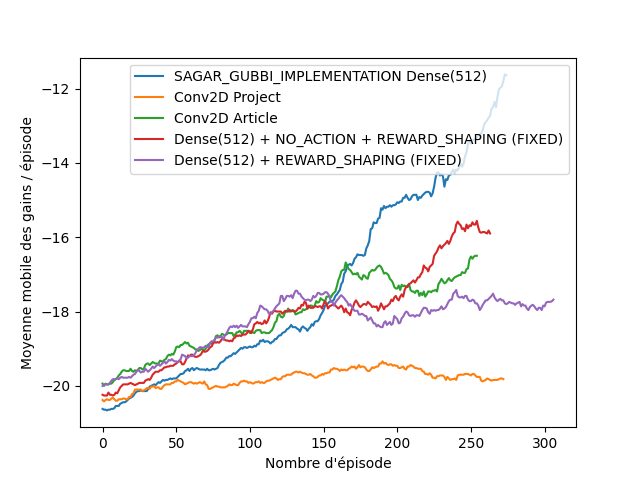
\includegraphics[width=0.5\textwidth]{rolling_average_graph.png}

\par Notre première modification a consisté à reprendre le même réseau de convolution que celui utilisé pour le projet Pong. 
Cependant, cette approche n'a pas été concluante. 
En effet, pour le projet Pong, nous avons utilisé un réseau convolutionnel avec un nombre restreint de 
paramètres. Nous avons pris cette décision car nous disposions d'un nombre limité de données labellisées 
et voulions diminuer le risque de sur-apprentissage. 

\par Ensuite, nous avons choisit d'utiliser le réseau de convolution 
décrit dans l'article \emph{Learning to Play Pong using Gradient Learning}\cite{PongPolicyGradient}.
Celui-ci a donné de meilleurs résultats que le réseau de convolution de notre projet, cependant, il n'a pas surpassé 
les performances de l'implémentation originale.

